% Define document class
\documentclass{aastex631}
\usepackage{float}
\usepackage{amsmath}
\usepackage{hyperref}
\usepackage{bm}


\newcommand\twostep{two-step\xspace}
\newcommand\full{full-fledged\xspace}

% Begin!
\begin{document}

% Title
\title{\texttt{nuance}: Detection of planetary transits in the presence of correlated noise}

% Authorz list
\author{Lionel J. Garcia, Daniel Foreman-Mackey, Fran Pozuelos}

% Abstract with filler text
\begin{abstract}
    We present \texttt{nuance}, an algorithm to search for planetary transits in light curves featuring correlated noises, such as instrumental signals and stellar photometric variability. Simpler approaches consist in searching for transits in light curves cleaned from correlated noise, where only transit signals would remain. However, we show that commonly used detrending techniques strongly affect transits signal-to-noise, up to the point of no detection when the noise characteristics is close to that of the transits. Focusing on stellar variability, we explore the parameter space for which this degradation occur, and quantify its effect on variety of cases.
\end{abstract}

% Main body with filler text
\section*{Introduction}
\label{sec:intro}

Exoplanets, planets outside our solar system, are discovered at an ever-increasing rate. Beyond the study of their inner structure and atmosphere, they give a unique glimpse to extrasolar systems formation, dynamics, as well as being probes to understand exoplanets' host stars. This is particularly true for systems whose orbital plane is aligned with our line of sight, leading to observable planetary transits. Although these transit signals can be seen in the apparent flux received from their stars, they are often mixed with other astrophysical and instrumental signals.
% together referred to as \textit{correlated noise}. 
If they can be disentangled from these nuisance signals, transits offer a powerful way to detect exoplanets. However, disentangling these signals comes with many challenges. Due to their nature we will refer to these signal as correlated noises\\
Widely used transit-search algorithms (Box-Least-Square algorithms \cite{bls}) are capable of detecting transits on light curves only containing transits and white noise. Hence, 
the simplest way to find periodic transit signals is to first clean a light curve from nuisance signals before performing the search. This strategy is widely adopted by the community, both using physically-motivated systematics models like \cite{everest1, everest2}, or empirical filtering techniques, such as the ones described and implemented in \cite{wotan}. However, when correlated noises start resembling transits, this cleaning step (often referred to as \textit{detrending}) strongly degrades their detectability. In such cases, the only alternative to search for transits is to perform a full-fledged modeling of the light curve, including both transits and correlated noises, and asses the likelihood of the model to the data on a wide parameter space, an approach largely avoided due to its untractable nature. Nonetheless, \citealt{kovacs2016} ask the question: \textit{Periodic transit and variability search with simultaneous systematics filtering: Is it worth it?}. The latter study discards the general benefit of using a full-fledged approach, but it fails at exploring the light-curves characteristics for which it becomes necessary.\\

% While it might only represent a handful of systems, this cases are extremely valuable for the exoplanetary science community. First, variability may be associated with star-spots that can be probed with the help of planetary transits. A better understanding of these structures benefit both the study of stellar atmospheres and their concerning impact on planetary atmosphere retrievals. Second, the growing interest of the community for ultra-cool dwarf stars comes with observations featuring enhanced red noise, stellar variability and lower transit SNR. Hence, these hidden system are pristine.$
We present \texttt{nuance}, an algorithm using linear models and Gaussian processes (GP) to simultaneously search for transits while modeling correlated noise in a tractable way, such as instrumental signals and stellar photometric variability. In \autoref{issues}, we describe the issues inherent to the two-step approach described earlier, and study the parameter space for which commonly used detrending techniques degrade transit signals to the point of no detection. In \autoref{nuance} we describe the tractable full-fledged approach of \texttt{nuance}, and its implementation in an open-source Python package. In \autoref{simu} we asses the performance of \texttt{nuance} by computing the recovery of planetary transits injected into simulated light curves. In section 4, we use nuance in a case study, to detect a known planet observed by the T E S S but undetected by the TESS pipeline due to its light curve characteristics. In section 5, we use nuance to search for transits in a list of .... Finally, we conclude this paper by providing avenues for the improvement of nuance, from its advantage to search for transits in ground-based observations, to its potential for the detection of multi-planetary systems affected by transit-times variations.

\newpage
\section{The issue with coorelated noise and its detrending}\label{issues}
Two sources of correlated noise particularly justify the need for a detrending step before searching for transits: instrumental noises (such as telescope pointing errors) and stellar variability (induced by  pulsations or starspots). In this section, we discuss the impact of such correlated noises and their detrending on transits detectability. For simplicity, we will model transit signals using an analytic empirical model described in \citealt{protopapas} (see Annexe).\\ 

\subsection{The effect of correlated noise on transits detectability}

To study transits detectability, we will focus on the signal-to-noise (SNR) of a unique event, reduced to the simplified expression (\citealt{pont2006}, Equation 12):

\begin{equation}\label{eq:snr}
  SNR= \frac{df}{\sqrt{\frac{\sigma_w^2}{n} + \frac{\sigma_c^2}{N_{tr}}}}
\end{equation}

where $df$ is the relative transit depth, $n$ is the number of points within transit, $N_{tr}$ the number of transits (unity here since we consider a single transit), and $\sigma_w$ and $\sigma_c$ are the white and correlated noise standard deviations. To show the impact of correlated noise on transit detectability, we simulate a unique transit signal and compute its SNR using \autoref{eq:snr}, both in the absence and presence of correlated noise (\autoref{fig:issue1}).

\begin{figure}[H]
    \begin{centering}
        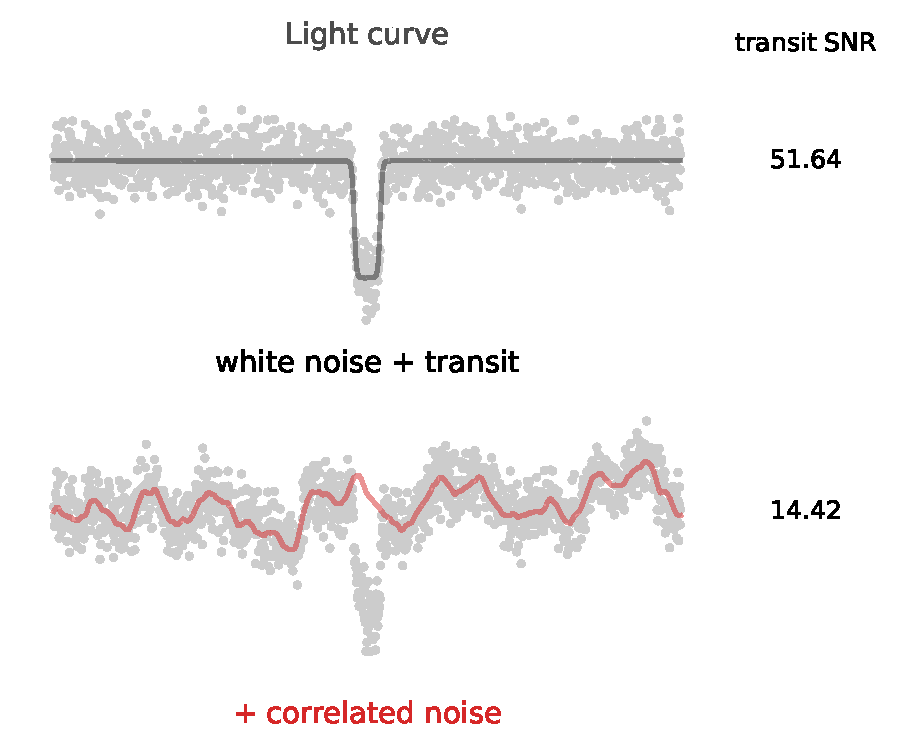
\includegraphics[width=8.5cm]{../figures/issue1.pdf}
        \caption{Illustration of the effect of correlated noise on a single transit singal-to-noise (SNR). A 1 hour transit of depth 1\% is simulated on top of white noise during a 24 hours observing window with an exposure time of 1 minute (top). Then, in the bottom plot, correlated noise is added to the transit signal and simulated using a Gaussian Process (GP) with a Matèrn-32 kernel of length-scale 1 hour and amplitude 0.2\%. The SNR on the right of each light curve is computed using \autoref{eq:snr}.}
        \label{fig:issue1}
    \end{centering}
\end{figure}

As illustrated in \autoref{fig:issue1}, the presence of correlated noise strongly decreases the transit signal SNR, limiting its detection. This issue rapidly motivated the development of systematics detrending algorithms such as the Trend Filtering Algorithm (\textsc{TFA}, \citealt{tfa}, in its primary use case), \textsc{SysRem} (\citealt{sysrem}), or Pixel Level Decorrelation (\textsc{PLD}, \citealt{pld}; see also \textsc{Everest} from \citealt{everest1, everest2}). Most of these methods rely on the shared nature of instrumental signals among light-curves (or neighboring pixels) such that the correction applied should not degrade the transit signal. We note that, except for \textsc{TFA}, these algorithms are mostly applied to space-based continuous observations, that provide continuous stellar baselines and mostly reproducible systematic signals. This is not the case for the vast majority of ground-based observations, in addition subject to periodic daytime interruptions and varying atmospheric extinction.

\subsection{The effect of detrending on transits detectability}

Instrumental signals have the benefit to be shared among light curves of stars observed with the same instrument, strongly correlated with measurements from the experimental setup (like detector's temperature, pointing error, sky background or airmass), hence we will make the strong assumption that their detrending based on an incomplete model of the light curve, one that ignore transit signals (because unknowns), do not affect the latter. In opposition, stellar variability is generally unknown and harder to correlate with simultaneous measurements. This gave rise to two types of treatments in order to reconstruct and detrend stellar variability, and perform transit search on \textit{flattened} light curves. One is physically-motivated and make use of Gaussian Processes (e.g. \cite{k2sc}). The other is empirical and make use of filtering algorithms (a wide variety being described in \cite{wotan}). In this section, we will study in details the effect of both approaches on transit detectability, by studying the degradation of a unique transit SNR for a wide variety of stellar variability characteristics.\\

Throughout this paper, we simulate stellar variability (and later model it) thanks to Gaussian Processes (GP), employing the physically-motivated stochastically-driven damped simple harmonic oscillator kernel (SHO) presented in \citealt{celerite1} (see Annexe ...). We generate stellar variability thanks to the \texttt{tinygp}\footnote{\href{https://github.com/dfm/tinygp}{https://github.com/dfm/tinygp}} Python package, providing an implententation of the scalable GP method from \citealt{celerite2} powered by \texttt{JAX}\footnote{\href{https://github.com/google/jax}{https://github.com/google/jax}}.

\begin{figure}[H]
    \begin{centering}
        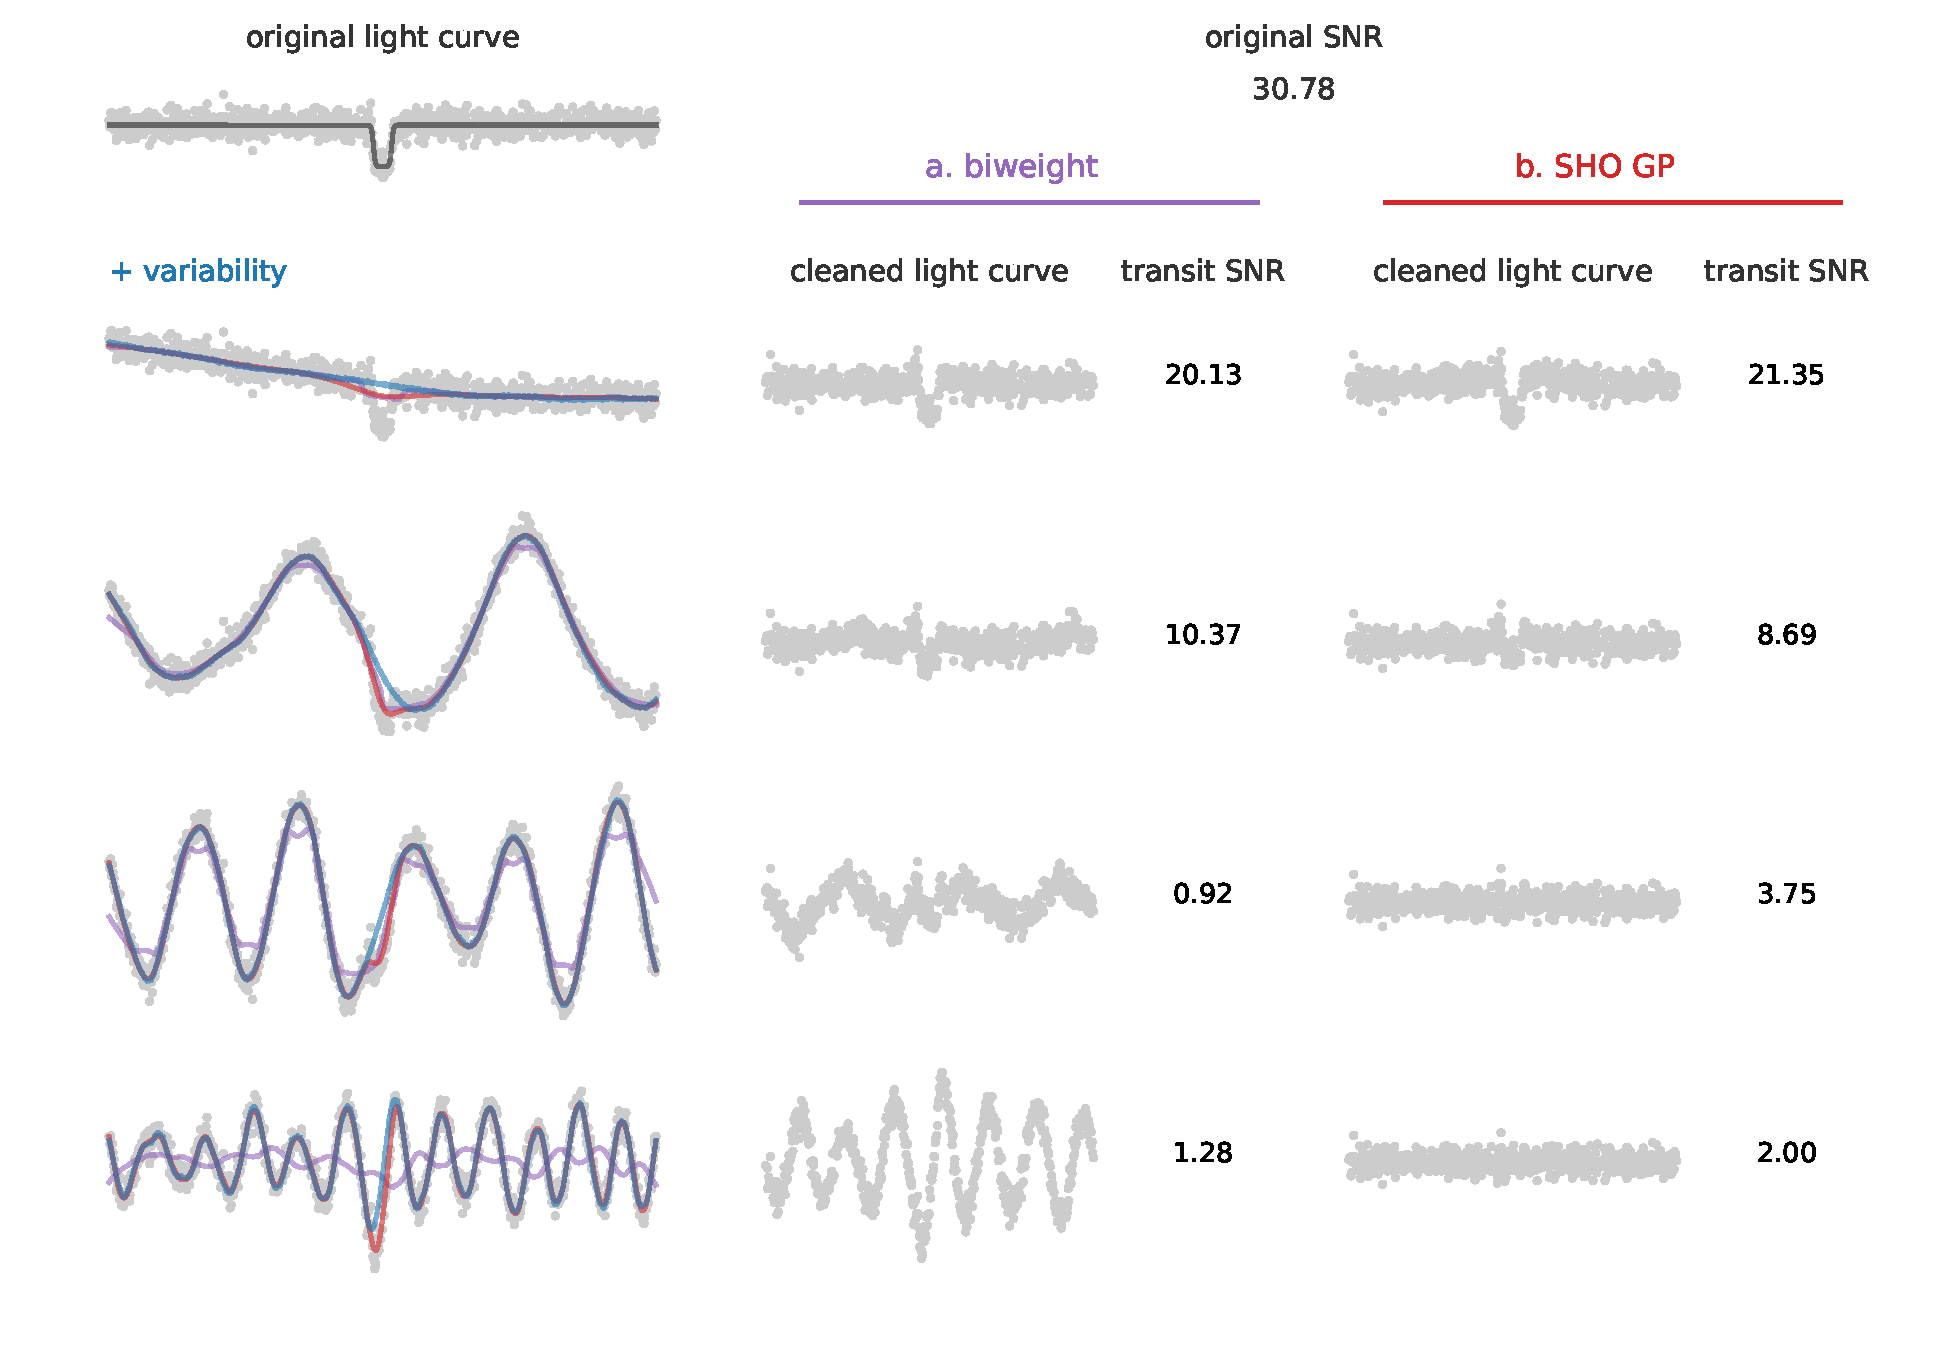
\includegraphics[width=\linewidth]{../figures/issue2.pdf}
        \caption{}
        \label{fig:issue2}
    \end{centering}
\end{figure}

In \autoref{fig:issue2}, we simulate a light curve featuring a single transit (again using the model from \citealt{protopapas}), in addition with stellar variability of different timescales and amplitudes. In case \textit{a} (purple in \autoref{fig:issue2}), we model and detrend these signals using the widely-adopted Tukey's biweight filtering method presented in \citealt{tukey} and its implementatation from \texttt{wõtan}\footnote{\href{https://github.com/hippke/wotan}{https://github.com/hippke/wotan}} \citep{wotan}. In case \textit{b} (red in \autoref{fig:issue2}) we employ the same GP model used to simulate stellar variability to reconstruct and remove it from light curves ignoring the presence of potential transits (the case of unknown transits search). Once transits cleaned from stellar variability, we asses their remaining SNR using \autoref{eq:snr}.\\

\autoref{fig:issue2} clearly shows the effect of both detrending techniques on transits SNR, and suggests that this degradation is strongly dependant on the stellar variability characteristics encountered. In order to explore the parameter space for which detrending is the most problematic, we simulate light curves including a single transit and a much wider range of correlated noise characteristics defined with two parameters: $\tau_v$ the relative timescale of the variability with respect to the transit duration; and $\delta_v$, the relative amplitude of the variability against transit depth, such that:

\begin{equation}
    \tau_v \propto \frac{\mathrm{variability\; timescale}}{\mathrm{transit\;duration}} \quad \text{and} \quad 
    \delta_v \propto \frac{\mathrm{variability\; amplitude}}{\mathrm{transit\;depth}} 
\end{equation}

To follow this parametrization, we simulate the photometric variability using a GP with an SHO kernel with hyperparameters \footnote{}:

\begin{equation}\label{eq:params}
    \omega = \frac{\pi}{\tau_v\tau} \quad 
    \sigma = \delta_v \frac{\delta}{2} \quad  \text{and}  \quad  
    Q = 10
\end{equation}

with $\delta$ and $\tau$ the depth and duration of the simulated transit, similar in all light curves. We fix a relatively high value for the quality factor $Q$ in order to restrict our simulations to strongly periodic variability signals. For $\tau_v=1$ and $\delta_v=1$, the expressions of $\omega$ and $\sigma$ given in \autoref{eq:params} correspond to a periodic signal with a period half that of the transit duration, and a peak to peak amplitude two times that of the transit depth, i.e. strongly resembling the simulated transit signal. As in \autoref{fig:issue2}, we reconstruct the variability using a biweight filter with a window length of $3\tau$ (three times the transit duration, an optimal value according to \citealt{wotan}). We then subtract the variability from each light-curve, estimate the resulting transit depth (using the in-transit minimum flux) and compute its SNR. \autoref{fig:snr_detrend} shows the remaining SNR values of transits computed this way, after each variability signals with random $(\tau_v, \delta_v)$ have been detrended.
% \bigskip\\
\begin{figure}[H]
    \begin{centering}
        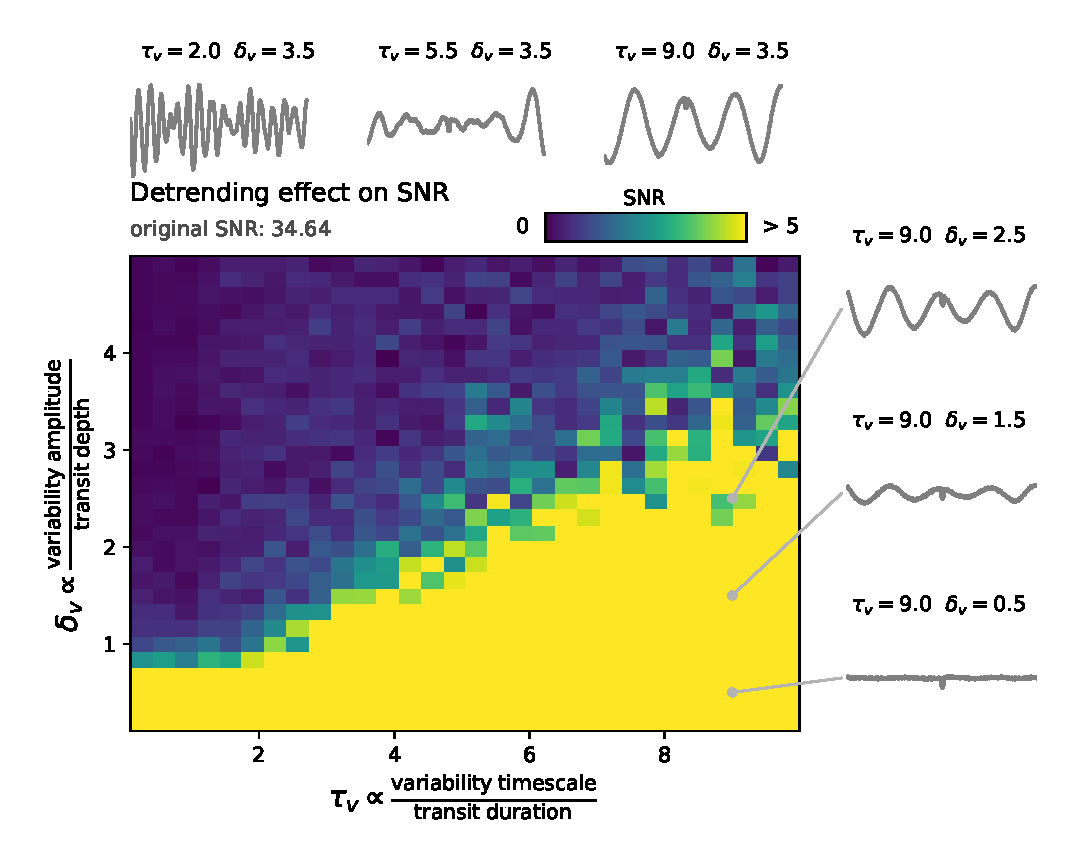
\includegraphics[height=9cm]{../../workflows/cleaning_snr/figures/simu1/result.pdf}
        \caption{}
        \label{fig:snr_detrend}
    \end{centering}
\end{figure}
\autoref{fig:snr_detrend} shows that it exists an entire region of the $(\tau_v, \delta_v)$ parameter space for which detrending degrades transit SNR to the point of no detection ($SNR < 6$). While this region might only represent a fraction of existing exoplanetary systems, we argue that these systems are of great value for the field of exoplanetary science. First, as variability is often linked to the presence of starspots, systems whose  with the stellar photo in is likely to be observed on stars whose equatorial plane lines up with our line of sight, following recent studies on the dynamical evolution of planetary systems \cite{}, hence being most likely to be transited. As a direct consequence, these same starspots are more likely to be occulted by planetary companions, events whose measurement benefits both the study of stellar atmospheres and their concerning impact on planetary atmospheric retrievals \cite{}. Finally, the growing interest of the community for ultra-cool dwarf stars comes with observations done in the infrared, featuring enhanced red noise and variability, leading to lower transit SNR \cite{}. Hence, commonly-used detrending technique (such as the biweight filter studied in this section) make transit-search blind to those pristine systems, motivating the need for a more informed transit search algorithm able to deal with correlated noises. In the next section we present such an algorithm: \texttt{nuance}.

\newpage
\section{\texttt{nuance}}\label{nuance}

In this section we describe \texttt{nuance}, an algorithm to search for planetary transits in light curves featuring correlated noises, such as instrumental signals and stellar photometric variability. Our approach is based on \cite{foreman2016}, developed to detect planetary transits accounting for a linear model of systematics in K2 light curves. \texttt{nuance} differs by modeling the covariance of the light curve with a gaussian process, accounting for correlated noise (especially in the form of stellar variability) while keeping the model linear and tractable.\\

\subsection{Preamble}

The flux $f$ of a star measured at time $t$ is sampled and aranged in the $(1\times N)$ column-vector $\bm{f}$. This flux contains instrumental signals, stellar variability and a periodic transit signal that we wish to uncover. An example of such signal is simulated and shown in \autoref{fig:principle_dataset}.

\begin{figure}[H]
    \begin{centering}
        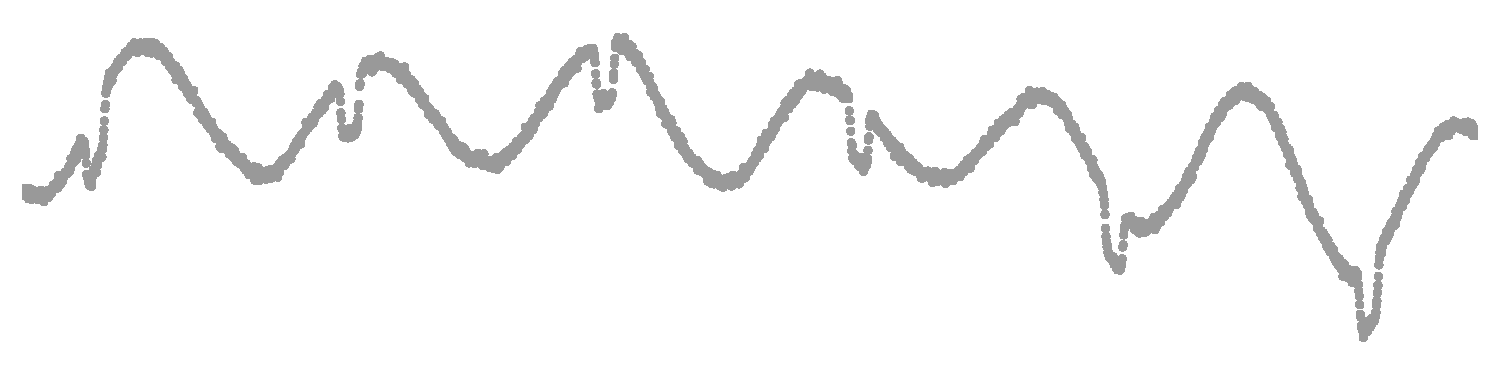
\includegraphics[width=0.7\linewidth]{../figures/principle_dataset.pdf}
        \caption{}
        \label{fig:principle_dataset}
    \end{centering}
\end{figure}

Simultaenously to the flux measurement, we obtained a set of $K$ measurements, aranged in the $(K\times N)$ matrix $\bm{X}$, that can be treated as explanatory variables for $\bm{f}$. Details about the simulation of these signals are provided in \autoref{app_principle_simulations}.
\\\\
Ideally, we would detect such  a periodic transit signal by sampling the posterior likelihood of this data to a full-fledged model including stellar variability (more generally correlated noises), instrumental systematics (modeled with explanatory variables), and a periodic transit signal of period $P$, epoch $T_0$, duration $D$ and depth $\Delta$. We would then reduce this posterior likelihood to $p(\bm{f}\vert P)$, its marginalized version over all parameters except the period $P$, producing a transit search periodogram. However, this approach has two issues: It is highly untractable, and it may lead to multimodal distributions that are hard to interpret.
\\\\
Given a period $P$, we instead want to compute the likelihood of a periodic transit signal at the maximum likelihood parameters $T_0$, $D$ and $\Delta$, i.e the periodogram

$$\mathcal{Q}(P) = \max_{T_0, D, \Delta}p(\bm{f} \vert P, T_0 ,D, \Delta)$$
\\
We will do that by adopting the strategy of \cite{foreman2016}, and separate the transt search into two components: the \textit{linear search} and the \textit{periodic search}. During the \textit{linear search}, the likelihood of a single non-periodic transit is computed for a grid of epochs, durations and depths. Then, the \textit{periodic search} consists in combining these likelihoods to compute the likelihood of a periodic transit signal for a range of periods. These combined likelihoods yield a transit-search periodogram on which the periodic transit detection can be based.


\subsection{The linear search}

During the linear search, the goal is to compute the likelihood of a single non-periodic transit signal of epoch $T_0$, duration $D$ and depth $\Delta$, for a grid of epochs, durations and depths, i.e.

$$\{p(\bm{f} \vert T_i ,D_j, \Delta_k)\}_{i, j, k}$$

To account for correlated noises, we model the light curve $f$ as being drawn from a Gaussian Process such that

$$\bm{f} \sim \mathcal{N}(\bm{w X}, \bm{\Sigma})$$

with mean $\bm{wX}$ (i.e. a linear model of the K explanatory variables with coefficients $\bm{w}$) and covariance $\bm{\Sigma}$. We include the non-periodic transit signal of epoch $T$, duration $D$ and depth $\Delta$ to our model by adding it as the last column of the design matrix $\bm{X}$, so that the transit is part of the linear model and the transit depth $\Delta$ can be solved linearly. Under this assumption, the log-likelihood of the data to the model, including a single non-periodic transit, can be computed analyticaly

$$\ln p(\bm{f} \vert \bm{X}) = -\frac{1}{2}(\bm{f}-\bm{wX})^T\bm{\Sigma}^{-1}(\bm{f}-\bm{wX}) -  \frac{1}{2}\vert\bm{\Sigma}\vert - \frac{K}{2}\ln 2$$


and the linear search is reduced to the computation of the latter log-likelihood over a grid of epochs and durations only, i.e.\footnote{In what follows, $\Delta_k$ is ommited from the notations, being linearly solved for any $(T_0, D)$}


$$\{\ln p(\bm{f} \vert T_i ,D_j)\}_{i, j}$$


Figure \autoref{fig:linear_search} shows this likelihood grid computed for the simulated dataset shown in \autoref{fig:principle_dataset}. To compute this grid, we used the same Gaussian Process and design matrix $\bm{X}$ used to generate the data (see annexe).



\begin{figure}[H]
    \begin{centering}
        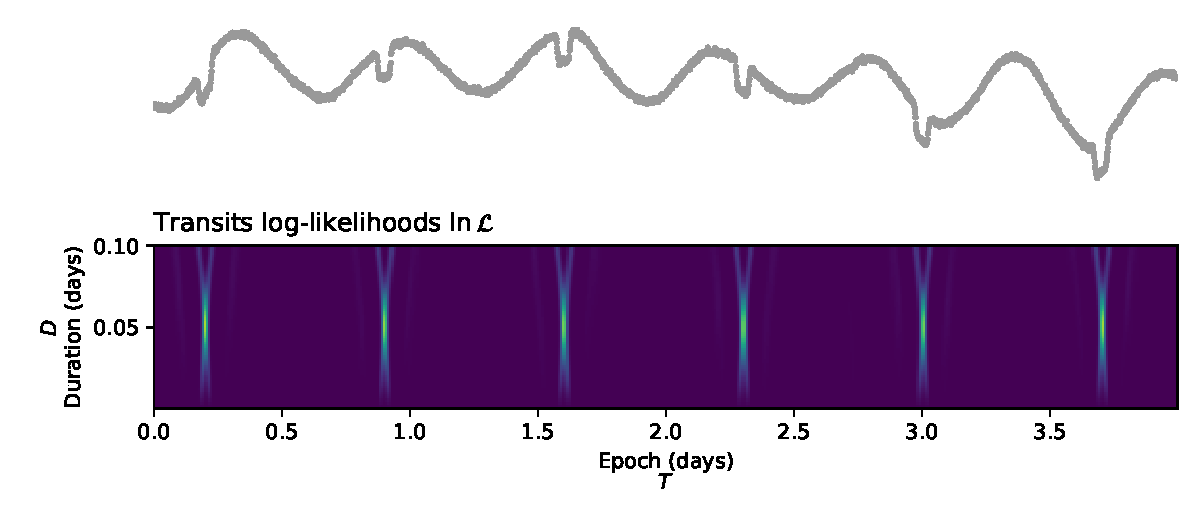
\includegraphics[width=0.75\linewidth]{../figures/principle_linear_search.pdf}
        \caption{}
        \label{fig:linear_search}
    \end{centering}
\end{figure}


\subsubsection{The periodic search}

We then need to combine the likelihoods computed from the linear search to obtain\footnote{Since we search for the maximum likelihood of $p(\bm{f}\vert...)$, we ommit $\bm{w}$ from the remaining notatitions, being linearly solved and taken at its maximum likelihood value} 

$$\max_{T_0, D}p(\bm{f} \vert P, T_0 ,D)$$

If each transits were to be considered truly independant, we would have

$$p(\bm{f} \vert P, T_0 ,D) \sim \prod_k p(\bm{f} \vert T_k ,D_k)$$

where $T_k$ are the epochs matching ($T_0$, $P$) and $D_k$ the durations of the corresponding transits. However, doing so leads to two issues:
\begin{enumerate}

    \item Transits are not truly independant and, instead of having their own depths $\Delta_k$, should share a common transit depth $\Delta$. We show in Annexe that there is an analytical expression for the likelihood of a periodic transit signal of depth $\Delta$ whose individual transit depths $\Delta_k$ with error $\sigma_k$ have been measured independantly:

    $$p(y \vert P, T_0 ,D) =  \prod_k \frac{\sigma_k \bar\sigma \, e^{- \frac{\left(\Delta_k - \Delta\right)^{2}}{2 \sigma_k^{2} + \bar\sigma^{2}}}}{\sigma_k^{2} + \bar\sigma^{2}}$$
    
    $$\text{with} \quad  
    \frac{1}{\bar\sigma^2} = \sum_{k}\frac{1}{\sigma_k^2} \quad \text{and} \quad
    \Delta = \bar\sigma^2 \sum_{k}{\frac{\Delta_k}{\sigma_k^2}}$$
    
    \item Individual epochs $T_k$ matching ($T_0$, $P$) are not necessarly available in the grid of epochs $\{T_i\}$. In \cite{foreman2016} this is solved by using the nearest neighbors in the epochs grid. In \texttt{nuance}, we rather interpolate the likelihood grid from $T_i$ to $T_k$ (see \autoref{fig:periodic_search}).

\end{enumerate}

\begin{figure}[H]
    \begin{centering}
        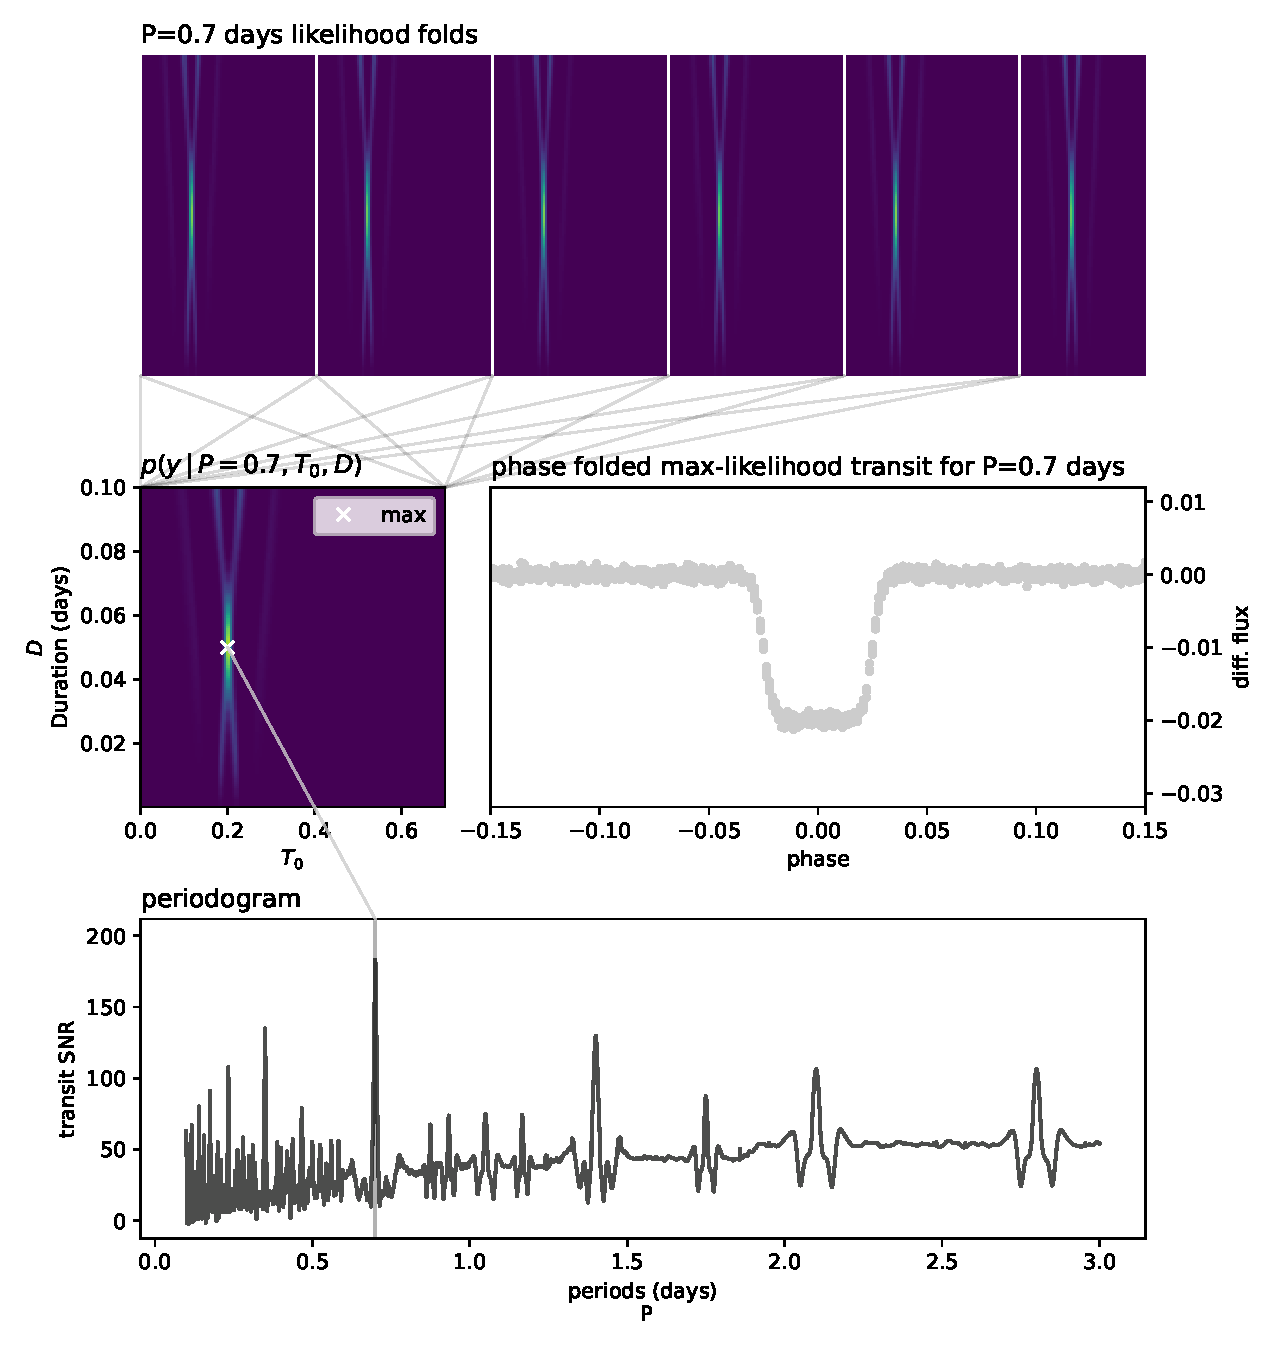
\includegraphics[width=0.8
        \linewidth]{../figures/principle_tiles_combined.pdf}
        \caption{}
        \label{fig:periodic_search}
    \end{centering}
\end{figure}

For a given period $P$, we can then compute $\max_{(T_0, D)}\{p(\bm{f} \vert P, T_0 ,D)\}$. But instead of relying on this maximum likelihood to build the final periodorgram, we compute the SNR of the transit with period $P$ and $(T_0, D)$ maximizing $p(\bm{f} \vert T_0 ,D, P)$, yielding the transit SNR periodogram shown in \autoref{fig:periodic_search}. We leave a discussion of this choice for Annexe .
\\\\
Once a transit recoverd, we mask the corresponding epochs in the log likelihood linear grid

\subsubsection{An open-source python package}


\section{Injection-recovery on simulated data}\label{simu}

\begin{figure}[H]
    \begin{centering}
        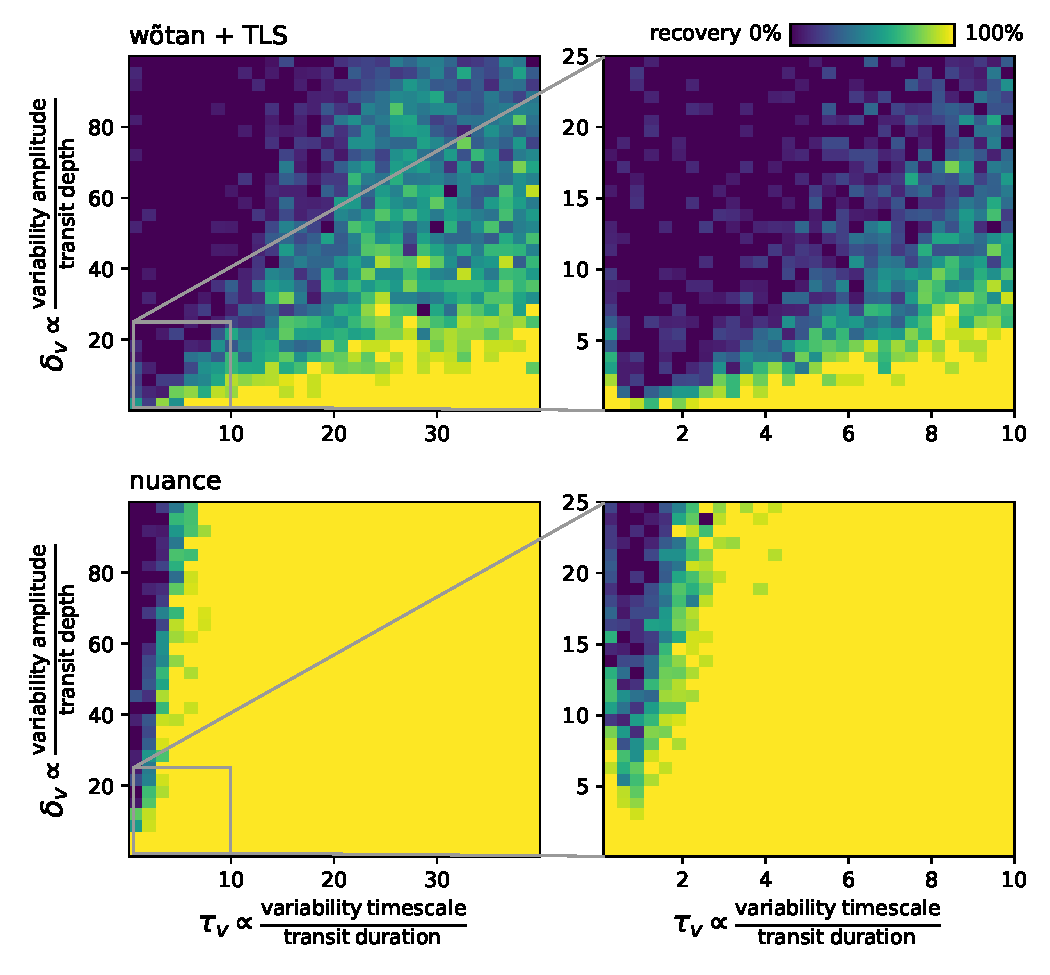
\includegraphics[height=12cm]{../../workflows/synthetic_injection_recovery/figures/final_result.pdf}
        \caption{}
        \label{fig:simu}
    \end{centering}
\end{figure}

\section{Comparison with \texttt{Sherlock} on TOI-540}\label{real}

\section{Performances and limitations}\label{perf}

\section{Conclusion}

This simulated dataset constits in a light curve featuring a transit signal of depth $1$\%, duration $0.05$ days and period $1.3$ days using the simple \citealt{protopapas} analytical model. It also contains a simulated variability signal drawn from a Gaussian Process with a quasiseparable 


\appendix
\section{Light curve simulations}\label{app_principle_simulations}
\bibliography{bib}

\end{document}
